\chapter{Blockchain in Business Sectors}
\label{ch:blockchain}

This chapter deepens the fundamentals of blockchain technology and explores its application in corporations. This helps to establish the base to analyze its potential impact on the auditing processes. 
Even though the main focus of this paper is the use of blockchain for auditing, it is important to 

\section{Fundamentals of Blockchain Technology}

\subsection{Introduction to Blockchain}
\label{Introduction to Blockchain}

Blockchain technology was first conceptualized as the subjacent architecture for a digital currency known as Bitcoin. This application was developed by an individual or organization not known by the public, under Satoshi Nakamoto's name, and published in a paper titled " A peer-to-peer electronic cash system" \cite{BTCWhitePaper}. During this thesis, the idea of this digital currency will not be argued, but it is important to remark on the broad implications that its underlying technology has had in every field, especially in accounting. However, even though Satoshi's approach was the first one to gain traction and started changing the course of the technology, it is not the first registered case of a blockchain. The first one can be attributed to Stuart Haber \cite{firstBlockchain} with the paper "How to time-stamp a digital document" in 1991 in which he proposed the main ideas that would be later converted into what is known now as blockchain. 

At its core, a blockchain is a further developed ledger that registers transactions in a computer network. However, the main catch is that it uses a distributed ledger, giving some extra characteristics to the data it processes such as increased safety, transparency, and immutability (Zibin Zheng \cite{attributesBlockchain}). Hence allowing participants of the network to agree on the state of a database without the need for a central authority. All this, with the intention of fomenting decentralization and trust in the system. 

This is an open technology, that everyone can adapt and build upon, which further increases its usability. However, there is an important distinction to make. As mentioned before, the word participant was used instead of user. The term participant has multiple meanings, such as the one given by the Cambridge Dictionary \cite{participantDefinition} "a person who takes part in or becomes involved in a particular activity". But for the sake of the paper, a participant will be understood as an individual or group that actively takes part in the maintenance of the blockchain. Verifying transactions and voting on their correctness. This, deeply differs from a user, as the second one would be the individual or organization that uses the blockchain, by adding transactions or receiving them. But without the need to interact with the Blockchain, or in some cases, know the technology nurturing the transaction whatsoever.

\subsection{Main components of every Blockchain}
\label{mainComponents}

A Distributed Ledger (DLT), also known as a distributed accounting book, it is a shared database, synchronized in multiple locations, usually geographically dispersed. Every individual or organization who wants to participate in the validation process of the distributed ledger, and therefore, the blockchain, has the ability to fork it and synchronize it with the rest of the network. 
Each participant or node is an exact copy of the ledger. This helps eliminate the problem of a single point of failure in the system and improves the reliability and resilience of the system. 

Another key component are the blocks and the transactions itself. The latter represents the fundamental operations registered inside any blockchain. A group of these transactions is called a block, which is later linked cryptographically to create a chain. Each block contains a group of transactions, a time stamp, a number of single-use, and a cryptographic hash of the former block, ensuring the integrity of the whole chain. In line manner, the hash function plays a critical role in the security of the data. The smallest of the changes in the input data produces a completely different chain of characters. As explained by Hongjun Wu \cite{hashFunctionDefinition}, it "enables to convert the key value to an address where the value is stored". It guarantees that any manipulation in the data will be easily detectable, as the hashes for the following blocks will not match. 

Nevertheless, any of this would work if it were not for the consensus protocol. These protocols are the way in which a blockchain decides what transactions or blocks get accepted into the blockchain. It enables participating nodes to append blocks as mentioned by Jie Xu \cite{consensusBlockchain}. The most typical consensus mechanisms are:
\begin{itemize}
        \item \textbf{Proof of Work:} The nodes, called miners, resolve complex (and resource-consuming) mathematical problems to validate transactions and create new blocks. This type of consensus consumes a lot of energy but gives increased security against bad actors. 
        \item \textbf{Proof of Stake:} The validators stake a part of their own tokens to participate in the creation of new blocks. If they act maliciously, they will lose it. This is a less secure but quicker and less energy-intensive type of consensus. 
\end{itemize}

\subsection{Types of Blockchain}

Multiple types of blockchains feed a diverse array of needs. The public option is the most present for financial public data, such as DLTs. However, public systems do not make the most sense for private entities such as multinational organizations as it would imply giving your competitors valuable operating data. The main types of blockchain are:
\begin{itemize}
    \item \textbf{Public Blockchains:} Open networks where \textit{participants} and \textit{users} have access to all information and the ability to add transactions to the network. There is not a single central entity or a consortium controlling it. They are completely decentralized and transparent. However, public blockchains face scalability issues and privacy problems (mainly in business-related activities).
    \item \textbf{Private Blockchains:} Contrary to the type below, this type of blockchain is controlled by an entity, and both \textit{participants} and \textit{users} have restricted access for its use and see. Being individually controlled carries some perks such as higher speeds and privacy, making them adequate for organizations. 
    \item \textbf{Consortium Blockchains:} Semi-decentralized and group-governed networks. It helps balance the benefits of decentralization but maintains some control. They are mainly used by groups or organizations that use the advantages of public data management while complying with regulations and operating efficiently. 
\end{itemize}

\subsection{Smart Contracts}
\label{sub: smart contracts}

Blockchain is not a single technology to implement, but it should be considered a system upon which to build. One of the main technologies created from it is smart contracts (SC). Concisely, SC can be described as an agreement that executes itself once certain criteria are met. In the words of Zibin Zheng et al. \cite{smartContractsDefinition}, "smart contracts enable the contractual terms of an agreement to be enforced automatically without the intervention of a trusted third party". 

As previously explained, smart contracts in auditing take a shift from retrospective approaches, in which auditing operations are conducted periodically and relying on sampling methods, into an approach more progressive or forward-looking approach. Each transaction executed via a smart contract is automatically verified and logged, creating an immutable and transparent record.
Hence, with this implementation in place, the auditor's role will be shifted more toward an analyzer than an accountant. Auditors will access the already verified data in real time and be able to monitor all the financial activities of a corporation. They will be seen more as an advisor. Contracts, as defined by the Merriam-Webster \cite{definitionContract} dictionary is a legally binding agreement between two or more parties that creates mutual obligations enforceable by law. The main implication comes from the elimination, or transformation, of trusted third parties, living that function to the smart contract itself. Thus, the role will be occupied more by software engineers than by accountants, at least till new large language models appear where accountants will be able to code, thus the function of understanding the accounting itself will popularize again. 

Furthermore, smart contracts can reduce human error while enhancing compliance. In every transaction around the world, certain criteria have to be met for it to occur. It could be a commercial transaction, in which the transaction is initiated once the supplier of the goods or services gives them to the consumer. Or there could be more requirements such as regulatory requirements or internal policies. For example, a smart contract can check before the transaction is even made, if a certain purchase adheres to some internal limit for the department (either for the product/service individually or for the sum of purchases in a period of time). Another example can be seen when distributing your employees' salaries, so they can be expended in compliance with tax laws and internal distribution packages. Even in shipping industries, where the standard can verify if the supplier complied with taxes and countries' regulations before releasing the transaction. 

However, the integration of smart contracts into auditing is not without challenges, the main one being the complexity of the contract itself. Traditional contracts, executed by humans, inherit the same capability that has made humans succeed, adaptability. In case of unforeseen circumstances, rapid changes, or even the swap of some variable in the real world, the algorithm cannot quickly transform and redesign. An example of this, where the information is not always verifiable instantly by the algorithm, could be the passing away of someone, which takes days to appear on the databases. Another function, not yet available in current working smart contract implementations for auditing is the sometimes need for discretion. Moreover, this is something relatively naive to implement. 
A critical consideration is the security and reliability of smart contracts. Blockchain technology, in general, is acclaimed as one, if not the most secure public transaction systems. However, this does not exclude it from malicious actors or problems inside the code. Flaws in the contract code can be exploited, leading to significant financial losses, as evidenced by incidents like the DAO hack \cite{DAOhack}. Nonetheless, some could argue that this is still the case for current technologies, which are constantly awestruck by hackers or exploiters. The only difference relies on the maturity of the technology. While traditional transaction technological systems have been tested and improved for decades, new blockchain and smart contract implementations are still new. 

Lastly, the widespread adoption of smart contracts in auditing may lead to operational and organizational challenges. Integrating smart contract-enabled systems with existing legacy systems can be complex and resource-intensive. Organizations need to manage the interoperability between new blockchain-based processes and traditional IT infrastructures. And this is not an easy task. For the moment, none of the existing systems is prepared to incorporate them.

\subsection{Main characteristics of blockchains}

\subsubsection{Security and immutability}

The security of the blockchain comes from its cryptographic foundations and decentralized architecture. On the transaction part, every transaction is secured by cryptographic hashing. As explained by Rajeev Sobti et al. \cite{hashingDefinition} hashing is "a function that compresses a string of arbitrary input to a string of fixed length”. Denoting, as explained before in \cref{mainComponents}, that it transforms every transaction into an irreversible output (hash) while making sure that the data keeps its integrity and authenticity. This means, not just that current transactions are secure, but that with time, every new block is formed and hash, their security improves even more, providing immutability.

In a pragmatic context, mistakes happen. Sometimes transactions get wrongfully accounted for, or some extra steps are required such as returns of goods, discounts, or many others. This is where different types of architecture for the distributed ledgers come into play. The architecture defines how the transactions get proposed and accepted, the rules or criteria to change them (or fix them), and the general characteristics of the systems like their privacy or autonomy. This is further discussed in (SECTION XXXXX). 

\subsubsection{Scalability and performance}

Scalability in multinational organizations always correlates with the ability of the auditing company to perform reliable scrutiny of the data. As explained in \cref{ch:intro}, they rely on sampling methods that consist of "taking a subset from chosen sampling frame or entire population" as cited by Hamed Taherdoost \cite{samplingDefinition}. Based on the quality of the internal control, the auditing company decides how big the sampling will be and how many transactions will be analyzed. However, in blockchain, scalability refers to a more technical term. Anamika Chauhan et al. \cite{scalability}, describes it as an issue that arises from the limited block size and the consensus mechanism that the blockchain uses. Both variables are adaptable to the system's needs when building it. It is a problem of whether every node will have enough time and resources to validate each transaction before it is included in the blockchain. This, technologically speaking, is feasible, as current blockchains for financial use, that handle thousands of transactions per second already have human-imperceptible latency, such as the Solana Network \cite{solana}. This is often challenged by the need for extensive computational work and data storage across decentralized networks. But, here, auditing environments play a crucial role, as all systems already in place follow a centralized architecture, downsizing the resources needed for its use. High transaction volumes can lead to problems such as network congestion, longer transaction times, and increased costs, limiting the use of blockchain for large-scale applications. Hence, one of the keys for this blockchain in auditing to work is its capacity to regulate transaction rate. Or in other words, to control who inserts transactions (such as in a centralized system). 

In addition, performance is closely related to scalability. It is measured by transaction throughput (transactions per second) and latency (transaction confirmation time). Likewise, is highly affected by its architecture, with block size and frequency of block creation being some of the main factors. However, this part gets tricky as both elements (transaction throughput and latency) and indirectly correlated. For instance, larger blocks can store more transactions but can take longer to propagate through the network, while smaller blocks enable faster validation but can limit throughput.



\section{Application of Blockchain in Organizations}

As clearly explained by Paul Brody, head of EY Global Blockchain \cite{ey_blockchain_explorer}, blockchain architecture is really reliable, but where things go wrong is in the interface between the blockchain and the real world. 

Currently, multiple companies are trying different implementations of blockchain in auditing. The Big Four (Deloitte, EY, PWC, and KPMG) are the ones with more skin in the game, creating usable applications. 
\begin{itemize}
    \item Deloitte: it has not created a functional application yet, but it has participated in multiple researches regarding this topic. They focused on its potential to transform traditional auditing methods. Highlighting the transparency and immutability that it can offer, and the importance of adapting audit methodologies to leverage blockchain’s capabilities.
    \item EY: it can be considered the leader among the four companies regarding its implementation of blockchain for auditing. Specifically, for the creation of the EY Blockchain Analyzer \cite{EYBlockchainAnalyzer}, a tool for assisting auditors in analyzing blockchain transactions and balances. This tool is further discussed in \cref{sub: EY case}.
    \item PWC: standing next to EY, they have also created a solution for auditing using blockchain called The Halo suite \cite{pwc_halo_cryptocurrency}. This tool enables auditors to ask questions to the blockchain. It helps facilitate the verification of transactions and balances and is available on multiple blockchains. 
    \item KPMG: their approach has been slightly different, focusing on a specific niche. On how blockchain can digitize and automate paperwork filings for the import and export of goods. It improves supply chain visibility, enabling all parties to securely and immutably submit and approve documents. This perse does not directly apply to auditing but has big indirect consequences on it as it improves information flow. 
\end{itemize}


At the forefront of all this research EY's and PWC's implementations stand out. Both tools implement usable and useful applications to interact with blockchain that facilitates the life of auditors. For the following chapter, the EY Blockchain Analyzer will be further analyzed:

\subsection{Case study - EY Blockchain Analyzer}
\label{sub: EY case}

EY is one of the largest auditing and consulting firms in the world, along with Deloitte, PWC, and KPMG \cite{ey_overview}. As of 2023, it has 395,442 employees in over 700 offices in more than 150 countries \cite{ey_revenue_record}. Given its size and market share, EY has the ability to invest in R\&D and create new products, that if implemented right, will move the market. 

The incursion of EY in blockchain is not something new. Their first paper "Blockchain reaction: Tech companies plan for critical mass" \cite{ey_first_paper} dives deep into how technology companies were preparing for blockchain’s widespread adoption. Since then, a lot has changed. Blockchain technology has improved along with EY's technical knowledge in the field. 

In their last approach, they created a tool called EY Blockchain Analyzer \cite{EYBlockchainAnalyzer}, intending to shrink the gap between auditors and this new technology. They tackle, with this tool, different problems that the industry was facing. For once they enable real-time auditing by unifying in the same platform, data flows from different sources such as blockchains, enterprise systems, and other data sets. With this innovation, they fixed two things at once. Information asymmetry, given that not all parties have access to all data sets. And bridging the gap between traditional systems and modern ones. A company would not be required to change its whole systems at once, but can, in fact, merge them into new ones for a cleaner transaction. 

Another key advantage is the inclusion of other blockchains either public or private. It accepts some of the biggest ones including Bitcoin, Ethereum, and Litecoin so reconciling information from all of them is not an issue. In addition, it is built in a way that makes its architecture modular, meaning that new blockchains and systems can be added as adoption grows. On the private part, it accepts independent networks such as Hyperledger Fabric \cite{hyperledger}, Quorum \cite{quorum_docs}, and private Ethereum instances.

Furthermore, it enables the execution of audit procedures. It can check whether transactions happened, or verify the balance of a wallet. It facilitates the auditing of transactions and it is integrated with EY's own platform (Helix \cite{ey_helix}), enhancing the ability to monitor transactions across on-chain and off-chain systems.

Currently, the tool is composed of three parts: Explorer \& Visualizer \cite{ey_explorer_visualizer}, Reconciler \cite{ey_reconciler}, Smart Contract \& Token Review \cite{ey_smart_contract_review}. The first one includes the basics like analyzing on-chain data for a given blockchain. It is connected to their own analytics infrastructure, being able to investigate semi-autonomously. Citing Paul Brody \cite{ey_blockchain_explorer} again, "Blockchains will do for a network of enterprises what ERP did for the single enterprise". The purpose of this part of the tool is to help corporations understand what is happening in their business. To be able to visualize the data on the blockchain and to make sense of it. This is an important part of the tool as it provides a human interface to understand all the data. For instance, raw transactions on a blockchain are represented in \cref{fig:etherscan}.

\begin{figure}[h!]
    \centering
    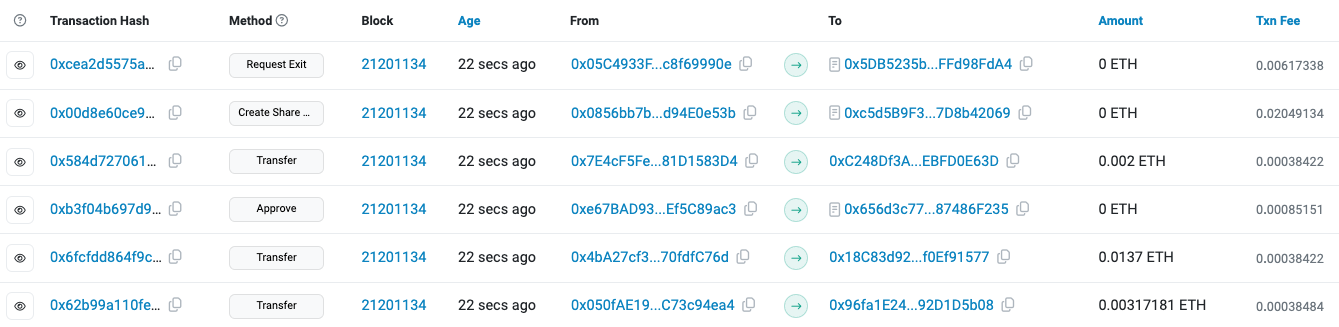
\includegraphics[width=1\linewidth]{include/Ethereum transaction.png}
    \caption{Screenshot of a random selection of transactions on the Ethereum blockchain using Etherscan \cite{etherscan}}
    \label{fig:etherscan}
\end{figure}

Every transaction is composed of a transaction hash a method, a block number, a timestamp, a sending address, a receiving address, an amount, and a transaction fee. In addition, is important to highlight that the block number is sequential and the wallet addresses are a random allocation of numbers and letters that look like this: 0x46df0faF9F30139E341D6082aa6b8992ad2f8D11.

As the reader may imagine, getting valuable insights from this information is not an easy task. To start with, the addresses are not humanly readable. That is where a visualizer comes into place. it helps to graphically represent every transaction coming in or from a wallet, demonstrating the connections. In addition, it has some other features like adding names to addresses or automatically marking transactions that meet certain criteria. \cref{fig:ey visualizer} represents an example of how the visualizer works given certain wallets. Every line marks a transaction and every figure a wallet. 


\begin{figure}[h!]
    \centering
    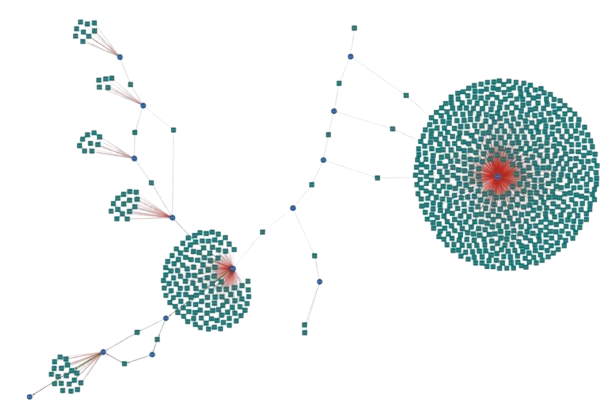
\includegraphics[width=0.5\linewidth]{include/EY visualizer 2.png}    
    \caption{Screenshot example of EY's Explorer \& Visualizer \cite{ey_explorer_visualizer}}
    \label{fig:ey visualizer}
\end{figure}

This helps drastically to see where transactions are flowing to and from to get a quick overview of the situation before diving deeper. This same technology could be applied to broader cases in multinational corporations, such as understanding how money flows between offices. This is not implemented in EY's tool, but Francesco Parino et al. \cite{btcCountryFlows} created a working representation (\cref{fig:btc flow}) of how bitcoin transactions flowed between countries in 2013.

\begin{figure}[h!]
    \centering
    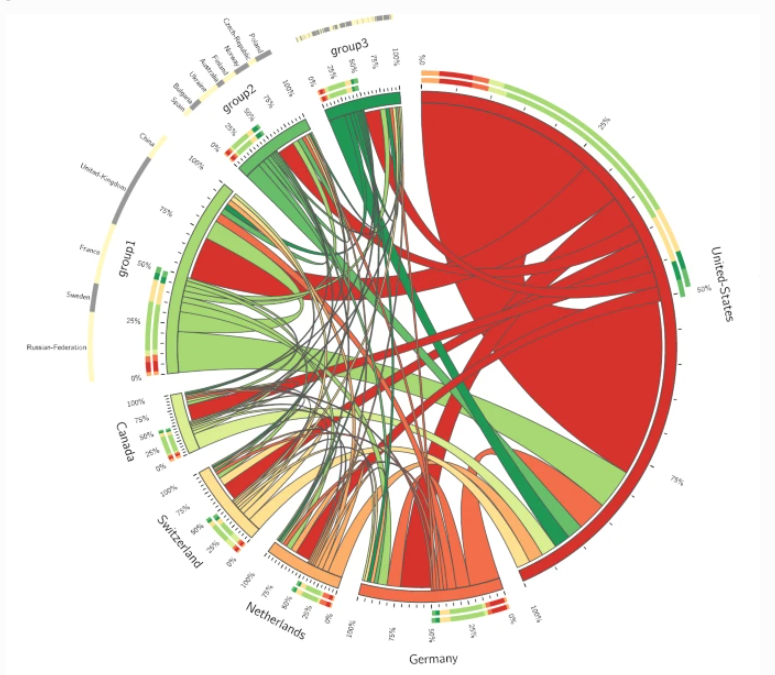
\includegraphics[width=0.6\linewidth]{include/BTC flow.png}
    \caption{Visualization of the international Bitcoin flow for 2013 by Francesco Parino et al. \cite{btcCountryFlows}}
    \label{fig:btc flow}
\end{figure}

A visualization tool like this, adapted for transactions between offices for example can provide quick and real-time insights into the flow of operations across regions. This could be used to clearly see real-time bottlenecks, inter-office dependencies, and optimization opportunities. An application of this could be the visualization of high transaction volumes between specific offices which may indicate potential areas for cost reduction. 

The second part of the tool discussed is the Reconciler \cite{ey_reconciler}. This tool intends to be used more as a checker than a creator. It verifies that all transactions are accounted for and accurately represented by matching client transaction data and wallet balances with the public blockchain ledger data. The idea is to skip third-party block explorers and fetch blockchain ledger data directly. This helps with the integrity of the data and reduces potential risks associated with implementing external applications. It also has the ability to verify digital signatures to confirm ownership of wallets which is critical for proving that an entity controls the digital assets being audited. Following EY's Blockchain Analyzer principles, it accepts data from on-chain and off-chain external systems and accepts multiple blockchains. 

Finally, the last tool implemented in the artifact is the Smart Contract \& Token Review. As Avner Geifman, EY's Blockchain Product Manager \cite{ey_smartContrat_cite} explains, "companies and individuals have to be confident that they can trust the code". This tool is added to verify smart contracts and increase confidence. As mentioned in \cref{sub: smart contracts} smart contracts are a key part of most blockchain systems. However, auditing them is difficult if you are not a software engineer. They are mostly composed of big code files, not readable by the inexpert eye. Having a tool that analyzes them and ensures they have no security flaws is a key part of making blockchain audits mainstream. Auditors do not have the time nor the ability to focus on that. The tool can check the Functionality, Security, and Quality of the smart contract. It can also execute the smart contract on a demo view to ensure it is reliable and give the auditors an idea of what to expect on-chain.  

In conclusion, even though the technology is as new as it can get, and has a lot of useful characteristics, is not quite there yet. There are a few challenges that they still have to overcome in order to make the technology mainstream. I've divided them into 6 blocks regarding their nature: Technical, Regulatory, Financial, Cultural, Security, and Governance.

\begin{itemize}
    \item \textbf{Technical challenges:} As with any new system or application, technical difficulties will always arise. In the specific topic of blockchain for auditing, there are two different types of challenges: the ones that come from the blockchain architecture (scalability, security, privacy), and the ones that come from the integration with the legacy systems. Regarding the first ones, a deeper dive will be given in XXXXX. On the other hand, the former has to deal with complex, established IT infrastructures. Legacy systems are systems written a long time ago, that due to coding and technical constraints at the time they were built, did not prioritize structure, maintenance, or understandability (Jane Ransom \cite{legacySystemsDefinition}). With time, as new improvements in memory systems, concurrency, or even the creation of new coding languages appear, these systems become more of a burden than a gift. As Keith Bennett puts it, "program understanding becomes a major maintenance activity" \cite{legacySystemsProblem}. The problem is that all of the existing legacy systems may not support the interoperability required for seamless data exchange with blockchain platforms. Meaning that these tedious systems would have to be updated once again. Which will take time and a lot of resources. This integration complexity can delay implementation and increase costs, making widespread adoption challenging.
    \item \textbf{Regulatory barriers:} The main regulatory burdens this technology faces can be categorized into two sections: existing regulation, and regulation to be made. As blockchain technology is relatively new and has not yet become widely adopted, regulators have not created legislation for it. As more implementations appear, and people start getting used to it, governments will begin creating new regulations, adding limits and responsibilities. In addition, multinational corporations operate in multiple jurisdictions, meaning that something that may be legal in one country, does not have to necessarily be allowed in the other. Each jurisdiction has its own set of regulations governing data privacy, financial reporting, and blockchain usage, among others. This lack of standard practices between regulations may delay the adoption of blockchain technology for auditing, as multinational companies prefer investing in technology that can be widely used across all their offices. \\
    Furthermore, regarding current regulations, data privacy, and in general terms, confidentiality is an important part of it. The inherent transparency of blockchain, even though it may be beneficial for auditing and data understanding, poses a big challenge to confidentiality. Not everyone can see all the data. For example, a participant of the blockchain who merely added an economic transaction should not be allowed to see the movement of money of the company. The big challenge here is to make sensitive financial data recorded on the blockchain inaccessible to unauthorized parties. But, so far, the technology is not quite there yet. In addition, the European Union (EU), where most multinational operations are located, is known for having strong protective data. For example, in the EU, one of the most important privacy regulations is the General Data Protection Regulation (GDPR) \cite{GDPR}. This regulation is meant to unify and strengthen in some cases, data protection laws for individual users inside the EU. Its goal is so that users have more control over their personal information, and applies to any entity that processes personal data of EU citizens, regardless of where the entity is located. This means that if they do not follow the rules, they can not operate within EU territory or with EU clients. This, as the reader may expect, difficult blockchain for auditing implementation not just in Europe, but throughout the world. Multinational corporations will not invest heavily in this technology if they are not able to deploy it in the biggest consumer market in the world. 
    \item \textbf{Financial constraints:} Fund allocation inside companies is one of the main impact areas for management. A drastic change in technology like adding blockchain to the auditing process, requires fund allocation not only for the acquisition or development of the tool but also for integrating it with existing systems and training employees. This big chunk of money completely deters small and medium companies from implementing the changes. Specifically, firms with tight budgets or stakeholders constrain them a lot, as this change in the tool will certainly not provide a big return on investments. In addition, employees will need to get educated in regards to how to use the new system effectively. All of them, as their auditing careers demonstrate, have extensive knowledge of accounting and auditing, but lack the technological expertise to understand the blockchain data, and get insights from the transaction movements. \\
    Another cost derives from the legal counsel. The technology is new and the regulation is not quite there yet. Companies have to be armored against any possible future attack regarding the confidentiality of the data they treat. Failing to comply with regulations can result in fines, legal action, or reputational damage, which also have their own financial repercussions. In the case of multinational corporations, this problem doubles in size as multiple jurisdictions are taken into place. Anu Bradford, explains in her paper "How the EU Became a Global Regulatory Power" \cite{EUsuperpowerRegulatorExample}, firms that operate in multiple jurisdictions, with different regulations and changes based on their interest, the smart move for companies is to adopt the most restrictive one among the big ones. Acting based on it in all the other regulations, even if they are not required to do so. This brings two main advantages. On the one hand, it reduces the burden of internal bureaucracy, as companies only have to adapt to one regulation, freeing a lot of resources and working power. On the other hand, in the possible and probable scenario in which the rest of the countries adopt similar regulations, they will already be prepared. As explained by Iris Benöhr \cite{consumerProtectionEvolution}, fundamental rights and consumer protection tend to improve over time. 
    \item \textbf{Cultural resistance:} 
    This topic is always a controversial aspect of implementing changes inside organizations. Employees are used to doing things in a certain way and tend to not enjoy changing them. This apprehension can lead to a lack of engagement with the new system, which can later end up in underperformance or underutilization of the capabilities of the system. Negativity in adapting to something comes from the failure to anticipate its efficiencies. \\
    These problems worsen given the misconceptions surrounding blockchain, and the initial complexity of understanding it. Given all this, it would be critical for companies to create tools that do not seem as if they were powered by blockchain. This would ease the transformation and appease people. However, this is not only a problem that average employees will face but is an issue at the managerial level too. Without strong support from management, initiatives to implement new technologies often struggle to gain traction.
    \item \textbf{Security issues:} While blockchain is inherently secure due to its decentralized and cryptographic nature, its applicability in tools for auditing may inhibit it from those exact features. Even in an hypothetic situation in which those attributes were still in place, it would not be immune to security challenges. Particularly, smart contracts are double-edged swords, as even though they provide one of the system's main advantages, self-executing contracts with the terms directly written into code are particularly vulnerable to errors or fraud. It requires a deep understanding of coding distributed networks to get a sense of what the smart contract is doing, provoking plenty of security concerns. Another security flaw appears when integrating it with legacy systems. These systems may already have some vulnerabilities in place that have not been discovered yet but when joining them with the new blockchain auditing systems, may provide new avenues for hackers to exploit. In addition, human factors are always the most insecure part of a system (Efthymia Metalidou et al. \cite{humanFactor}). Insider threats, whether intentional or accidental, have to always be accounted for. Even with robust access controls or training courses, these problems are still present in traditional blockchain systems. \\
    However, the main inconvenience of blockchain systems for auditing is that it is a new technology. With time and real errors, most problems will be solved eventually. Technology takes time to mature and gain strength, and with time, vulnerabilities become less and less common.
    \item \textbf{Governance difficulties:} This implies all the rules and processes for how decisions are made and enforced. It considers how the network operates and who has access to it. Defining the governance structure is the key to how all the data is going to be treated. Protocol updates, access rights, or data-sharing policies are all examples of how this can affect any tool implementing blockchain for auditing. In general, this is the part of the system that decides who has control over it, how decisions are made, and how any problem may be resolved. The flow of the data and the ability to change it are all important factors that should be decided before launching the blockchain. 
\end{itemize}

In summary, EY's application is a great first step towards a future where blockchain auditing is the norm. They have a deep understanding of the auditing profession and are making improvements to ease the way towards this blockchain implementation. The ability to visualize the blockchain facilitates a lot of the understanding of it. The tool specialized in analyzing blockchain transactions provides a useful tool for making sense of a large quantity of data. In addition, the smart contract reviewer is an incredible tool that will shorten the gap between auditors and software engineers, and let them interact more freely and safely within the blockchain.

However, there is still a lot of work to do. Financial constraints are still a huge problem, as stakeholders do not get any direct benefit from incorporating this technology over traditional systems. There is a good intention of not replacing legacy systems but working with them to draft down costs and ease the transition. Nevertheless, this same relation may cause other types of costs like legacy system maintenance and adaptability, new cybersecurity threads, and even technical challenges. In addition, regulation does not make it easier. Multinational companies tend to operate given the standards with the most strict rules out of the big consumer markets. This idea is still true in this situation, but there is not yet any specific regulation in place in any big economy, making the implementation of the technology more uncertain. Furthermore, culturally, the symbiotic relation between already-in-place systems and new blockchain tools for auditing, makes it easier for users to interact with the tool and spend less time in training. However, this is not of use if users do not fully understand the new abilities that blockchain offers. These new auditing tools create a new paradigm in which a deep understanding of the system is extremely beneficial to recognize patterns and transaction flows. 

So, even though EY's Blockchain Analyzer is a great start for the creation of new tools for auditing analyzing in real-time using blockchain, its implementation still faces plenty of challenges. Not all of them, though, can be controlled by the company, such as cultural resistance or regulatory barriers. But what can be said already based on the trajectory of the tool, is that it is becoming closer to a usable system in which the value added to it makes it worth it to use it over traditional ones. 

\section{Types of Blockchain Implementations for Auditing}

At its core, blockchain is a digital and distributed representation of a ledger with given characteristics such as immutability, transparency, or decentralization. But not all blockchains come in the same shape. This section delves into the different blockchain models and how can they be adapted to meet the needs of real-time auditing, examining how different implementations can address the challenges faced by multinational corporations.

\subsection{Blockchain architectures}

The usual and most talked about characteristic of blockchain is its decentralized network, meaning that there is not a single entity or person that controls it. Currently, as of 2024, blockchains are most visibly in digital currencies, providing a realistic other option to fiduciary money.  However, this is not always the case. For instance, as talked about in \cref{Introduction to Blockchain}, the first real use case of blockchain was in the New York Times newspaper \cite{firstBlockchain} as a private type of blockchain. 

These are just some examples of blockchain architecture but there are plenty more:

\begin{itemize}
    \item \textbf{Public blockchains:} They operate on a decentralized network where anyone can join and participate in the consensus process. The data produced on them is available to anyone, and all users can add and validate transactions. They are transparent and open, with the ability to adapt and update based on a voting system (F Irresberger et al. \cite{publicBlockchains}). Given that no private single entity has control over the entire system, they provide an immutable record of transactions. Only in the extreme case of a union with the majority of the power of the system, a transaction can be reversed. And even then, everyone will be aware of it and can solve it by forking the system \cite{forks}. This transparency and immutability result in higher trust in the system and an increased propensity to effectuate transactions without the sender and the receiver knowing each other. \\
    About its limitations, they tend to suffer slower transaction speeds and limited throughput. Also, as their name suggests, they are public and have an open nature, meaning that privacy is not an option.
    \item \textbf{Private blockchains:} As opposed to public blockchains, private ones are completely controlled by a single organization or individual. In the same way that private establishments reserve the right to accept clients, private blockchains have to accept participants to read or write transactions. In addition, the accepting part of the transactions is completely managed by the consensus process that the private entity decides to incorporate. The main key idea of this type of blockchain is that information produced inside of it, stays there. Sensitive financial data remains confidential within the organization, and only a selected number of individuals or other corporations may have access to it (which could be revoked later). Furthermore, this controlled environment offers higher transaction speed and processing which derive an improved scalability, ideal for private multinational corporations. On the other hand, the limitations have to do with its centralized system, with trust issues and a dependent reliance on a single entity that may introduce vulnerabilities such as a single point of failure or the potential for internal fraud.
    \item \textbf{Consortium blockchains:} This option is a mix of the two prior. It is a semi-decentralized network managed by a group of organizations. Several entities get together to form it and no single organization has any power to accept transactions or changes without the support of some others. The consensus is achieved through a set of pre-selected nodes, balancing the need for privacy with collaborative control. Shared infrastructure and resources can lower costs of creation and maintenance, as well as improve security and enhance auditing processes. On the contrary, its limitations have to do with the same thing that highlights them as a suitable option for organizations. The governance is complex as there are a lot of interested parties that may not always share the same vision. The possibility of the formation of cartels that rule over the other members. 
    \item \textbf{Hybrid blockchains:} The idea is similar to the consortium blockchains, of mixing private and public attributes, but instead of being done by multiple entities, everything is organized under just one. Initially, all data generated in the blockchain is public and accessible to everyone, but the corporation can make private certain parts of the system and restrict access only to pre-authorized people or entities, such as in the case of an audit. It is a combination of public trust with private control. In addition, by controlling data visibility, corporations can better adhere to legal requirements regarding data privacy and disclosure. Conversely, the creation and maintenance of a blockchain with these characteristics requires more work than the rest. Robust protocols have to be in place and cybersecurity measures well thought as to private parts of the system remain private.
\end{itemize}
    
\subsection{Deployment models}

\subsection{Consensus mechanisms}

